\documentclass[aspectratio=169]{beamer}
\usepackage{graphics,amssymb,amsfonts,amsmath}
\usepackage{pgf,tikz}
\usetikzlibrary{shapes,shapes.geometric,positioning,trees}
\DeclareGraphicsExtensions{.jpg,.pdf,.mps,.png}
\usepackage[latin1]{inputenc}
\usepackage[brazil]{babel}
\usepackage[normalem]{ulem}
\usepackage{standalone}
\usepackage{pgfpages,enumerate,hyperref}
\usepackage{palatino}   %Fonte sem serifa.
\usepackage{ragged2e}   %Par\'agrafo justificado.
\usepackage{minted}
% \usetheme{CambridgeUS}
% \usetheme{AnnArbor}
% \usecolortheme{lily}
\usecolortheme{orchid}
\usefonttheme[onlymath]{serif}

%colocando n\'umero de p\'aginas no slide.
\setbeamertemplate{footline}[frame number]

% desativando os botoes de navegacao.
\beamertemplatenavigationsymbolsempty

%Tela cheia
\hypersetup{pdfpagemode=FullScreen}

% Layout da p\'agina
\hypersetup{pdfpagelayout=SinglePage,urlcolor=blue,colorlinks=true}

% Ambiente bash
\newminted{bash}{bgcolor=gray}

% Ambiente python
\newminted{python}{bgcolor=green!25!white}

\tikzstyle{every node}=[anchor=west]
\tikzstyle{selected}=[draw=red,fill=green!30]
\tikzstyle{optional}=[dashed,fill=gray!50]

\title{Tutorial Django 1.8}
\author{R\'egis da Silva {\texorpdfstring{\color{blue}}{ }@rg3915}\\ e\\ Jayme Neto \texorpdfstring{\color{blue}}{ }@kalkehcoisa}
\institute{Grupy-SP}
\date{\today}

\begin{document}
\justifying %Par\'agrafo justificado.

%Neste caso insere somente no primeiro slide.
{%
%\usebackgroundtemplate{\centering \vspace*{5cm} \includegraphics[width=\paperwidth]{figuras/djangoPython}}

\usebackgroundtemplate{%
\vbox to \paperheight{\vfil\hbox to \paperwidth{\hfil
\includegraphics[width=\paperwidth]{img/logo_mascote.jpg}\hfil}\vfil}
}

\begin{frame}

\end{frame}
}

\begin{frame}
	\titlepage
\end{frame}

\begin{frame}[fragile]
	
Se tiver pressa...

\begin{bashcode}
	$ git clone https://github.com/rg3915/django1.8.git
	$ virtualenv -p python3 django1.8
	$ cd django1.8
	$ source bin/activate
	$ make initial
	$ ./manage.py runserver
\end{bashcode}

... sen\~ao, leia o tutorial.

\end{frame}

\begin{frame}\frametitle{Ementa}

\begin{itemize}
	\item MTV e ORM
	\item 1 min de Python
	\item Instala\c c\~ao
	\item Criar o ambiente
	\item Criar o projeto e a App
	\item Deploy no Heroku
\end{itemize}

\end{frame}

\begin{frame}\frametitle{Objetivo}


\begin{itemize}
	\item Criar uma lista de filmes
	\item Retornar o filme de maior bilheteria
	\item Criar um formul\'ario
	\item Ver os detalhes de cada filme
\end{itemize}

\end{frame}


\begin{frame}\frametitle{O que \'e Django?}

Segundo Django Brasil,

\

\begin{exampleblock}{}
	{\it Django \'e um framework web de alto n\'ivel escrito em Python que estimula o desenvolvimento r\'apido e limpo.}
\end{exampleblock}

\end{frame}

\begin{frame}\frametitle{O que \'e Django?}

\begin{itemize}
	\item adota o padr\~ao MTV
	\item possui ORM
	\item admin
	\item heran\c ca de templates e modelos
	\item open source
\end{itemize}

\end{frame}

\begin{frame}\frametitle{Quem usa Django?}

	\begin{figure}[h]
	  \centering
  		
\includegraphics[height=.7\paperheight]{img/eu_uso_django}
	\end{figure}

\begin{center}
\url{www.djangosites.org}
\end{center}


\end{frame}


\begin{frame}\frametitle{Sites}

\begin{enumerate}
	\item \url{www.djangoproject.com/}

	\item \url{www.djangobrasil.org/} (desatualizado)

	\item \url{www.djangopackages.com/}

	\item \url{www.groups.google.com/forum/django-brasil}

	\item \url{www.pythonclub.com.br/}

	\item \url{www.github.com/rg3915/django-basic-apps}

	\item \url{www.realpython.com/blog/categories/django/}

	\item \url{www.marinamele.com/taskbuster-django-tutorial}
\end{enumerate}

\end{frame}



\begin{frame}\frametitle{MVC x MTV}

\begin{itemize}
	\item {\bf Model} - \'e o modelo, a camada de abstra\c c\~ao do banco de dados, onde acontece o ORM
	\item {\bf View} - \'e o controlador, onde acontece as regras de neg\'ocio e a comunica\c c\~ao entre a base de dados e o navegador
	\item {\bf Templates} - \'e a camada de apresenta\c c\~ao, s\~ao as p\'aginas html
\end{itemize}

\end{frame}

\begin{frame}\frametitle{MVC x MTV}
	\begin{figure}[h]
	  \centering
  		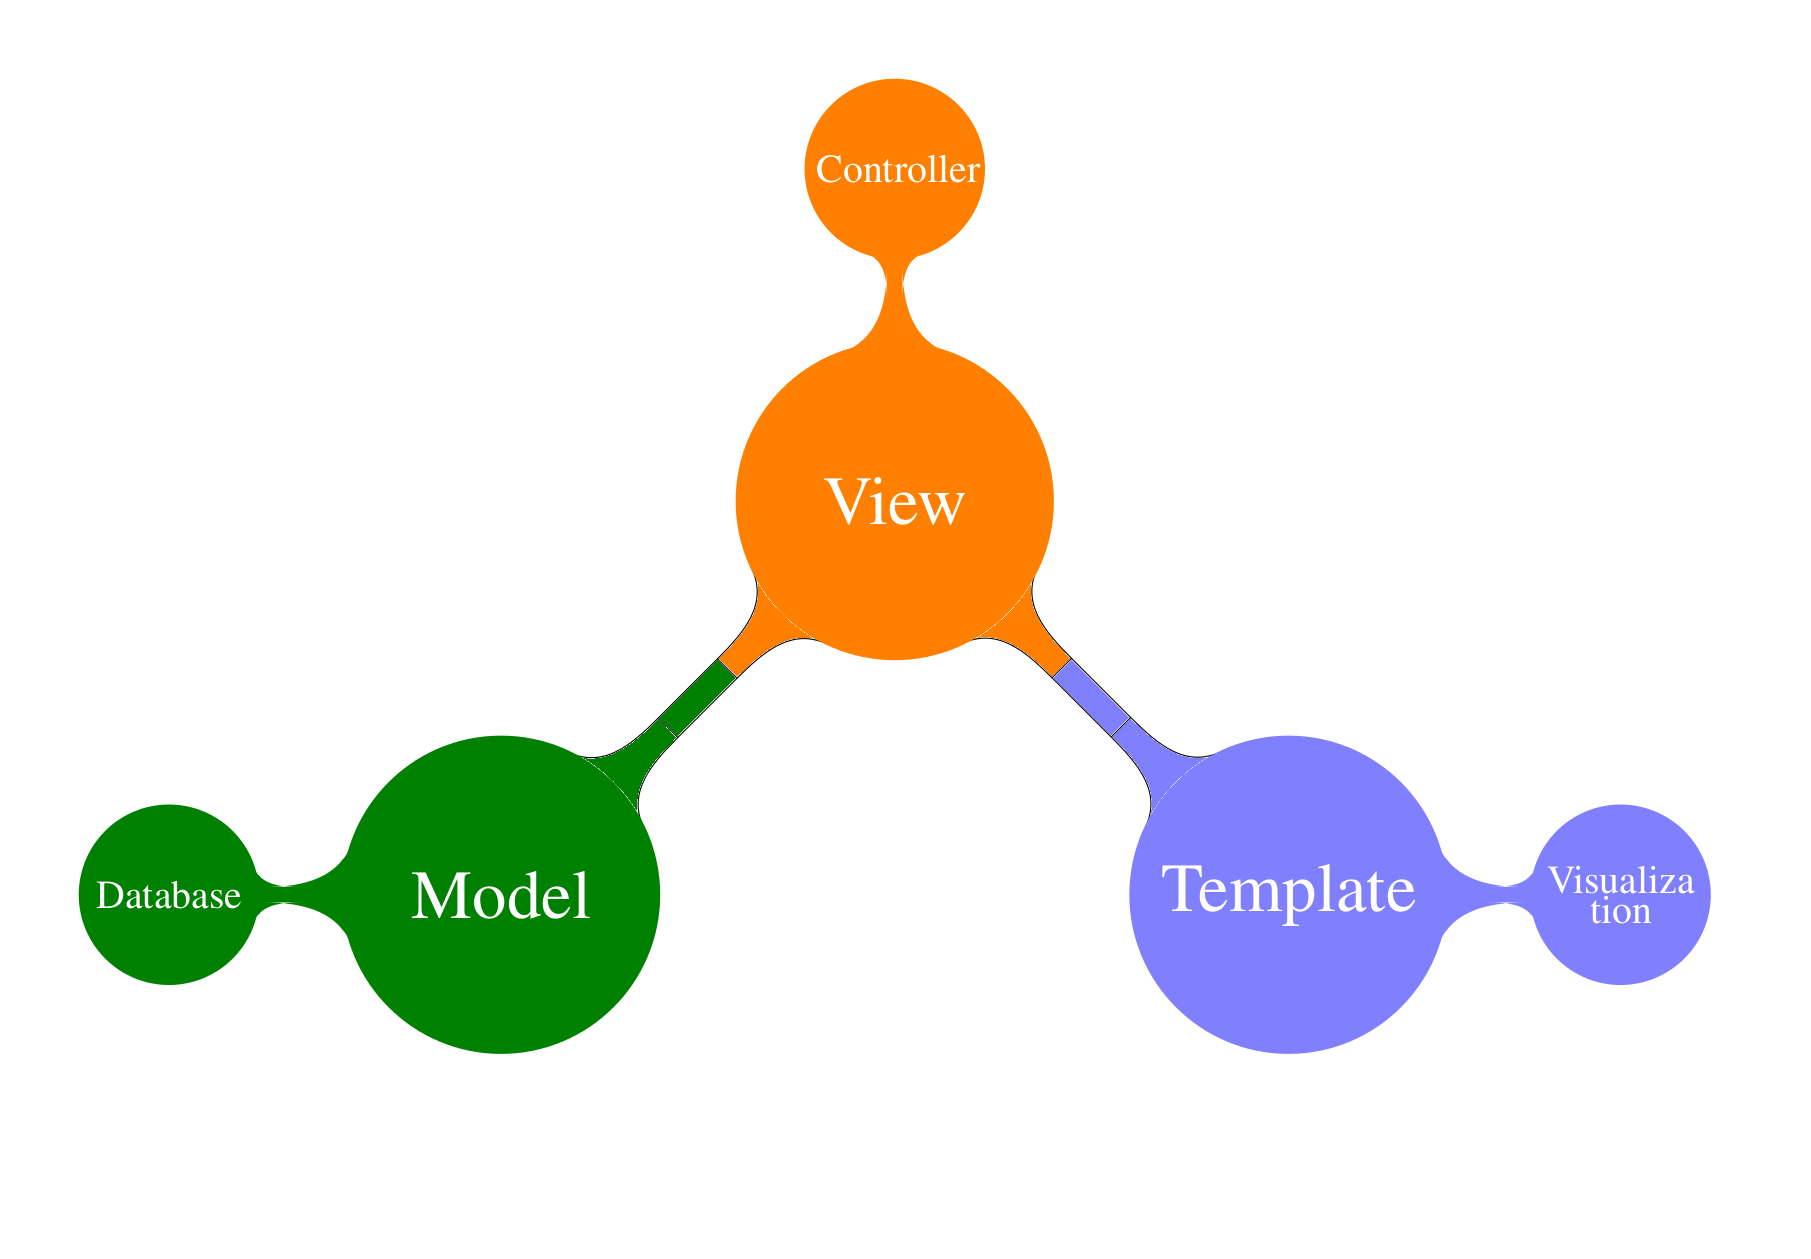
\includegraphics[height=.9\paperheight]{img/mtv1.png}
	\end{figure}
\end{frame}

\begin{frame}\frametitle{MVC x MTV}
	\begin{figure}[h]
	  \centering
  		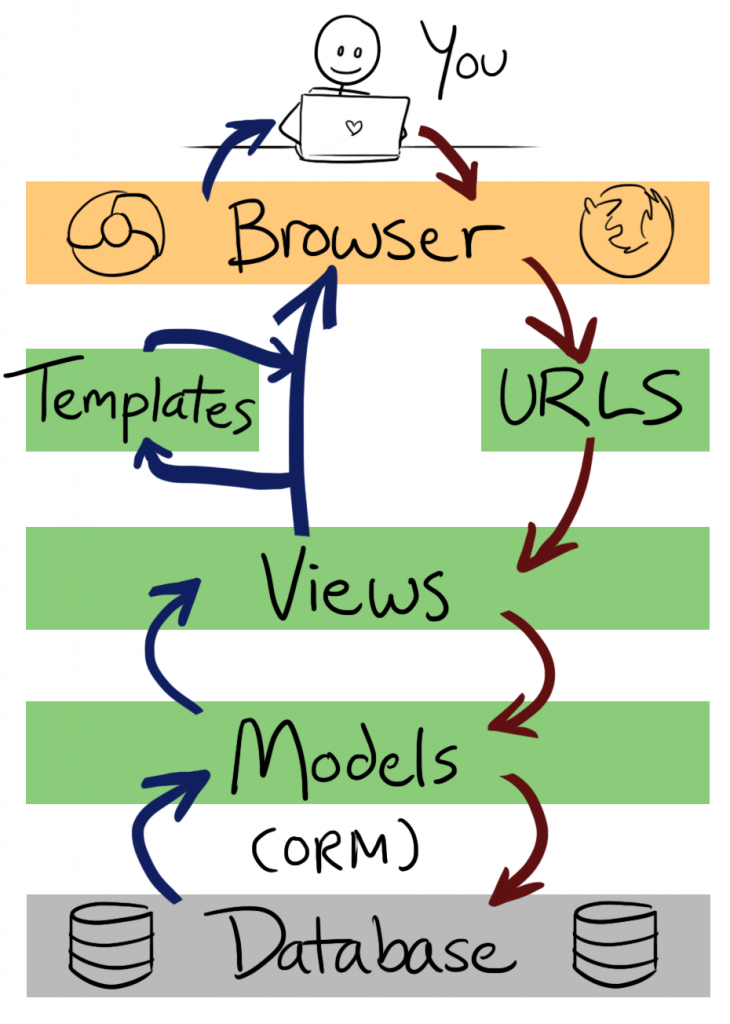
\includegraphics[height=.9\paperheight]{img/mtv2.png}
	\end{figure}
\end{frame}


\begin{frame}\frametitle{ORM}

\begin{itemize}
	\item Modelo (Classe) = Tabela
	\item Atributos = Colunas
	\item Objetos = Tuplas (Registros)
\end{itemize}

\end{frame}

\begin{frame}[fragile]\frametitle{1 min de Python}

\begin{pythoncode}
    public static void main (String[] args){
        System.out.println("Desculpa");
    } # oops

    print("Python") # simples assim

    def soma(a, b):
        return a + b

    soma(25,9)
\end{pythoncode}

\end{frame}

\begin{frame}[fragile]\frametitle{1 min de Python}

\begin{pythoncode}
    lista = ['a', 10, 5.5]
    for i in lista:
        print(i)

    for i in range(10):
        print(i)

\end{pythoncode}

\end{frame}

\begin{frame}\frametitle{O que voc\^e precisa?}

\begin{itemize}
	\item Python (2 ou 3)
	\item Pip
	\item VirtualEnv
\end{itemize}\textbf{}

\end{frame}

\begin{frame}\frametitle{Instalando Python no Windows}

\begin{itemize}
	\item Download do python: \url{https://www.python.org/downloads/windows/}
	\item Configurar as vari\'aveis de ambiente (PATH)
\end{itemize}

\textbf{Leia}: \textit{Instalando e Configurando o Python e Django no Windows} - Thiago Cor\^oa \url{http://pythonclub.com.br/instalacao-python-django-windows.html}

\

\textbf{Pip}
\begin{itemize}
	\item Gerenciador de pacotes do python
	\item \url{https://pip.pypa.io/en/latest/installing.html\#install-pip}
\end{itemize}

\end{frame}


\begin{frame}[fragile]\frametitle{Instalando no Linux}

\begin{itemize}
	\item \textbf{Pip} \url{http://pip.readthedocs.org/en/latest/}
\end{itemize}

Primeira op\c c\~ao

\begin{bashcode}
    $ wget https://bootstrap.pypa.io/get-pip.py
    $ sudo python get-pip.py
\end{bashcode}

Segunda op\c c\~ao

\begin{bashcode}
    $ sudo apt-get install -y python-pip
\end{bashcode}


\begin{itemize}
	\item \textbf{VirtualEnv} \url{https://virtualenv.pypa.io/en/latest/}
\end{itemize}

Digite

\begin{bashcode}
    $ sudo pip install virtualenv
    $ # ou
    $ sudo apt-get install -y virtualenv
\end{bashcode}

\end{frame}

\begin{frame}\frametitle{O que vamos considerar no nosso projeto?}

\begin{itemize}
 \item \Large{Ambiente: venv}
 \item \Large{Projeto: myproject}
 \item \Large{App: core}
\end{itemize}

\end{frame}

\begin{frame}[fragile]\frametitle{Criando o ambiente}

Vamos criar um ambiente usando o Python 3, ent\~ao digite

\begin{bashcode}
	$ virtualenv -p /usr/bin/python3 venv
\end{bashcode}

onde \textit{venv} \'e o nome do ambiente.

\

Entre na pasta

\begin{bashcode}
	$ cd venv
\end{bashcode}

\

e ative o ambiente

\begin{bashcode}
	$ source bin/activate
\end{bashcode}

\

Obs: todos os pacotes instalados com o ambiente ativado ser\~ao instalados dentro do ambiente e vis\'iveis somente nele.
\end{frame}

\begin{frame}[fragile]
\textbf{Dica}: No Linux, edite o arquivo \textit{$\sim$/.bashrc}

\begin{bashcode}
	alias sa='source bin/activate;'
\end{bashcode}

\

Assim voc\^e cria atalhos para ativar seus ambientes:

\begin{bashcode}
	$ sa
\end{bashcode}

\

\textbf{Dica}: Para diminuir o caminho do prompt digite

\begin{bashcode}
	$ PS1="(`basename \"$VIRTUAL_ENV\"`):/\W$ "
\end{bashcode}

\

O caminho vai ficar assim

\begin{bashcode}
	(venv):/venv$
\end{bashcode}

\

Onde \textit{(venv)} \'e o nome do ambiente e \textit{:/venv\$} \'e a pasta atual.

\

Para desativar o ambiente digitamos

\begin{bashcode}
	(venv):/venv$ deactivate
\end{bashcode}


\end{frame}

\begin{frame}[fragile]\frametitle{Instalando Django 1.8 + django-bootstrap-form}

\begin{bashcode}
	$ pip install django==1.8.4 django-bootstrap-form
\end{bashcode} 

\

\url{https://github.com/tzangms/django-bootstrap-form}

\

Vendo o que foi instalado

\begin{bashcode}
	$ pip freeze
	Django==1.8.4
	django-bootstrap-form==3.2
\end{bashcode}

\

\

Crie o \textit{requirements.txt} (os ingredientes do bolo)

\begin{bashcode}
	$ pip freeze > requirements.txt
\end{bashcode}

\end{frame}

\begin{frame}[fragile]\frametitle{Criando o projeto e a App}

\url{https://docs.djangoproject.com/en/1.8/intro/tutorial01/}

\

Para criar o \textbf{projeto} digite

\begin{bashcode}
	$ django-admin.py startproject myproject .
\end{bashcode}

\

repare no ponto final do comando, isto permite que o arquivo \textit{manage.py} fique na pasta "principal", pasta \textit{venv}.

\end{frame}

\begin{frame}[fragile]

Criando a \textbf{app}

\begin{bashcode}
	$ python manage.py startapp core
	ou
	$ ./manage.py startapp core
	ou
	$ manage startapp core
\end{bashcode}

\

\

\textbf{Dica}: para funcionar o \'ultimo comando voc\^e deve editar o \textit{$\sim$/.bashrc}

\begin{bashcode}
	$ alias manage='python $VIRTUAL_ENV/manage.py'
\end{bashcode}

\

O que temos at\'e aqui?

\begin{bashcode}
	$ tree myproject; tree core
\end{bashcode}

\end{frame}

\begin{frame}[fragile]

\begin{tikzpicture}[%
  grow via three points={one child at (0.5,-0.7) and
  two children at (0.5,-0.7) and (0.5,-1.4)},
  edge from parent path={(\tikzparentnode.south) |- (\tikzchildnode.west)}]
  \node {.}
    child { node {manage.py}}
    child { node [selected] {myproject}
      child { node {\_\_init\_\_.py}}
      child { node [optional] {settings.py}}
      child { node [optional] {urls.py}}
      child { node {wsgi.py}}
    }
    child [missing] {}				
    child [missing] {}				
    child [missing] {}				
    child [missing] {}				
    child { node [selected] {core}
      child { node [optional] {admin.py}}
      child { node {\_\_init\_\_.py}}
      child { node [optional] {models.py}}
      child { node [optional] {tests.py}}
      child { node [optional] {views.py}}
    };
\end{tikzpicture}

\end{frame}


\begin{frame}[fragile]\frametitle{Django funcionando em n\'ivel 0}

Criando a primeira migra\c c\~ao

\begin{bashcode}
	$ python manage.py migrate
\end{bashcode}

\

\textbf{Obs}: o comando \texttt{migrate} se chamava \texttt{syncdb} e s\'o era capaz de criar novas tabelas no banco de dados. J\'a o \texttt{migrate} consegue remover e alterar tabelas. Criado baseado nas funcionalidades do Django South.

\

Rodando o projeto

\begin{bashcode}
	$ python manage.py runserver
\end{bashcode}

\

Por padr\~ao ele est\'a rodando na porta 8000

\url{http://localhost:8000/} ou \url{http://127.0.0.1:8000/}

ou

\begin{bashcode}
	$ python manage.py runserver <PORTA>
	$ python manage.py runserver 8080
\end{bashcode}

\url{http://localhost:8080/}
\end{frame}


\begin{frame}

	\begin{figure}[h]
	  \centering
  		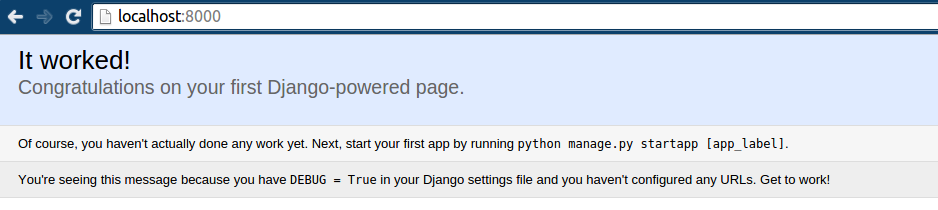
\includegraphics[width=.9\paperwidth]{img/it_worked.png}
	\end{figure}

\end{frame}

% \begin{frame}

% ### Django South

% * Detecta alterações nos models.py e gera scripts para ajustar o banco de dados
% * Faz "versionamento" de bases de dados
% * Permite migra\c c\~ao de bases dados de um SGBD para outro

% \end{frame}


\begin{frame}\frametitle{O m\'inimo - n\'ivel 1: settings, views, urls}

\begin{tikzpicture}[%
  grow via three points={one child at (0.5,-0.7) and
  two children at (0.5,-0.7) and (0.5,-1.4)},
  edge from parent path={(\tikzparentnode.south) |- (\tikzchildnode.west)}]
  \node {.}
    child { node [selected] {myproject}
      child { node {...}}
      child { node {settings.py}}
      child { node {urls.py}}
    }
    child [missing] {}				
    child [missing] {}				
    child [missing] {}				
    child { node [selected] {core}
      child { node {...}}
      child { node {views.py}}
    };
\end{tikzpicture}

\end{frame}


\begin{frame}[fragile]\frametitle{Editando settings.py}

\begin{pythoncode}
	
	INSTALLED_APPS = (
	    ...
	    'core',
	)
\end{pythoncode}


\end{frame}


\begin{frame}[fragile]\frametitle{Editando views.py}

\begin{pythoncode}
	# -*- coding: utf-8 -*-
	# from django.shortcuts import render
	from django.http import HttpResponse

	def home(request):
	    return HttpResponse('<h1>Django</h1>
	                         <h3>Bem vindo ao Grupy-SP</h3>')
\end{pythoncode}

\end{frame}


\begin{frame}[fragile]\frametitle{Editando urls.py}

\begin{pythoncode}
from django.conf.urls import include, url

urlpatterns = [
    url(r'^$', 'core.views.home'),
    url(r'^admin/', include(admin.site.urls)),
]
\end{pythoncode}

\

Ou

\

\begin{pythoncode}
from django.conf.urls import patterns, include, url

urlpatterns = patterns(
    'core.views',
    url(r'^$', 'home'),
    url(r'^admin/', include(admin.site.urls)),
)
\end{pythoncode}

\end{frame}

\begin{frame}

	\begin{figure}[h]
	  \centering
  		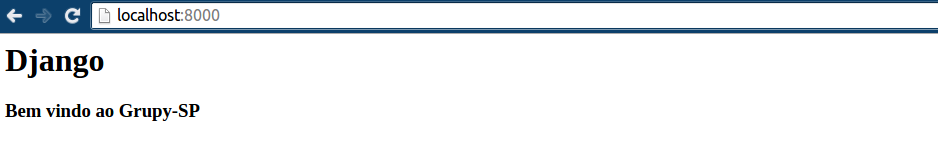
\includegraphics[width=.9\paperwidth]{img/HttpResponse.png}
	\end{figure}

\end{frame}

\begin{frame}[fragile]\frametitle{Admin}

\begin{bashcode}
	$ python manage.py createsuperuser --username='admin' --email=''
\end{bashcode}

\end{frame}

\begin{frame}

	\begin{figure}[h]
	  \centering
  		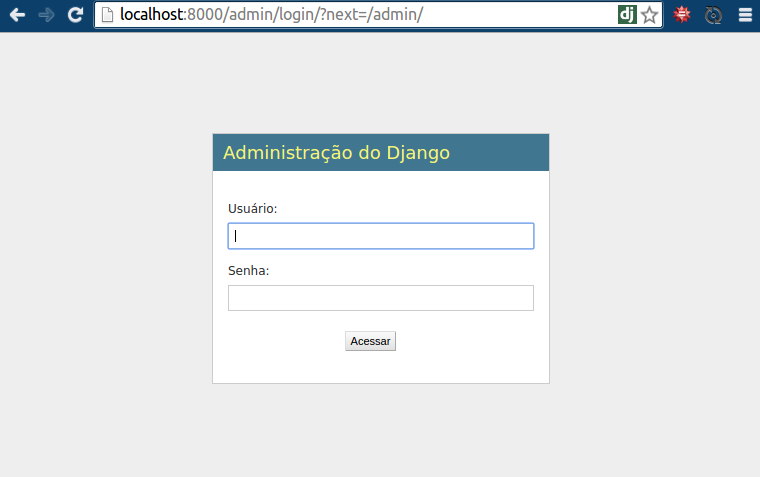
\includegraphics[height=.9\paperheight]{img/admin1.png}
	\end{figure}

\end{frame}

\begin{frame}

	\begin{figure}[h]
	  \centering
  		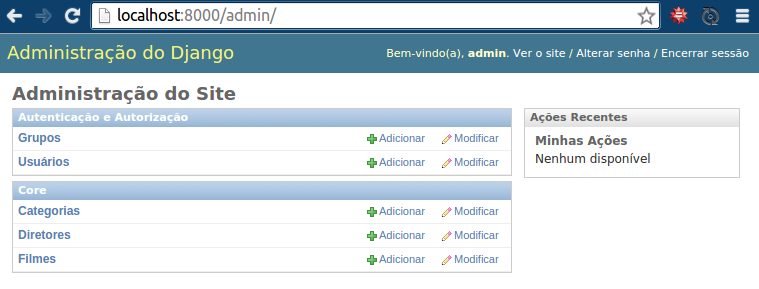
\includegraphics[width=.9\paperwidth]{img/admin2.png}
	\end{figure}

\end{frame}

\begin{frame}[fragile]\frametitle{Tocando o barco}

\textbf{Editando settings.py}

\begin{pythoncode}
	LANGUAGE_CODE = 'pt-br'

	TIME_ZONE = 'America/Sao_Paulo'

	LOGIN_URL = '/admin/login'
\end{pythoncode}


\end{frame}


\begin{frame}\frametitle{Testes}

	\begin{figure}[h]
	  \centering
  		
\includegraphics[width=.9\paperwidth]{img/teste03.png}
	\end{figure}

\end{frame}

\begin{frame}[fragile]

\textbf{Teste}: Verificar se existe a p\'agina \textit{index.html}.

\begin{pythoncode}
	from django.test import TestCase

	class HomeTest(TestCase):

	    def setUp(self):
	        self.resp = self.client.get('/')

	    def test_get(self):
	        ''' get / deve retornar status code 200. '''
	        self.assertEqual(200, self.resp.status_code)

	    def test_template(self):
	        ''' Home deve usar template index.html '''
	        self.assertTemplateUsed(self.resp, 'index.html')
\end{pythoncode}

\

\textbf{Leia}: \textit{pytest: escreva menos, teste mais} - Erick Wilder de Oliveira - \url{https://goo.gl/8E9FB1} 

\end{frame}

\begin{frame}[fragile]\frametitle{Editando views.py}

\begin{pythoncode}
	from django.shortcuts import render
	# from django.http import HttpResponse

	# def home(request):
	#     return HttpResponse('<h1>Django</h1><h3>Bem vindo ao Grupy-SP</h3>')

	def home(request):
	    return render(request, 'index.html')
\end{pythoncode}

\end{frame}

\begin{frame}[fragile]\frametitle{Criando o index.html}

Estando na pasta \texttt{venv} digite

\begin{bashcode}
	$ mkdir -p core/templates
	$ echo "<html><body><h1>Tutorial Django</h1>
	        <h3>Bem vindo ao Grupy-SP</h3></body>
	        </html>" > core/templates/index.html
\end{bashcode}


\end{frame}

\begin{frame}[fragile]\frametitle{Editando models.py - Filmes}

	\begin{figure}[h]
	  \centering
  		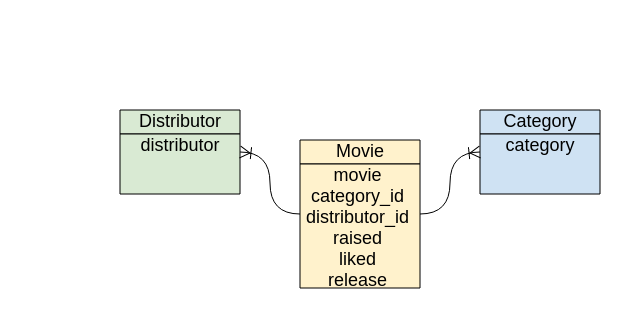
\includegraphics[width=.8\paperwidth]{img/diagram.png}
	\end{figure}

\end{frame}


\begin{frame}[fragile]\frametitle{Editando models.py}

\begin{pythoncode}
	# -*- coding: utf-8 -*-
	from django.db import models

	class Distributor(models.Model):
	    distributor = models.CharField('distribuidor',
	                                   max_length=50, unique=True)

	    class Meta:
	        ordering = ['distributor']
	        verbose_name = 'distribuidor'
	        verbose_name_plural = 'distribuidores'

	    def __str__(self): # ou __unicode__ no Python 2
	        return self.distributor
\end{pythoncode}

\end{frame}


\begin{frame}[fragile]

\begin{pythoncode}
	class Category(models.Model):
	    category = models.CharField('categoria',
	                                max_length=50, unique=True)

	    class Meta:
	        ordering = ['category']
	        verbose_name = 'categoria'
	        verbose_name_plural = 'categorias'

	    def __str__(self):
	        return self.category

\end{pythoncode}

\end{frame}


\begin{frame}[fragile]

\begin{pythoncode}
	class Movie(models.Model):
	    movie = models.CharField('filme', max_length=100)
	    category = models.ForeignKey(
	        'Category', verbose_name='categoria',
	        related_name='movie_category')
	    distributor = models.ForeignKey(
	        'Distributor', verbose_name='distribuidor',
	        related_name='movie_distributor')
	    raised = models.DecimalField(
	             'arrecadou', max_digits=4, decimal_places=3)
	    liked = models.BooleanField('gostou', default=True)
	    release = models.DateTimeField(u'lancamento')
	    class Meta:
	        ordering = ['-release']
	        verbose_name = 'filme'
	        verbose_name_plural = 'filmes'
	    def __str__(self):
	        return self.movie
\end{pythoncode}


\end{frame}

\begin{frame}[fragile]\frametitle{Tipos de campos}

\begin{minipage}[t]{.45\linewidth}
	\begin{itemize}
		\item BooleanField
		\item CharField
		\item DateField
		\item DateTimeField
		\item DecimalField
		\item DurationField
		\item EmailField
		\item FileField
		\item FloatField
		\item ImageField
	\end{itemize}
\end{minipage}
\begin{minipage}[t]{.45\linewidth}
	\begin{itemize}
		\item NullBooleanField
		\item PositiveIntegerField
		\item PositiveSmallIntegerField
		\item SlugField
		\item SmallIntegerField
		\item TextField
		\item TimeField
		\item ForeignKeyField
		\item ManyToManyField
		\item OneToOneField
	\end{itemize}
\end{minipage}

\

\

\url{https://docs.djangoproject.com/en/1.8/ref/models/fields/}

\end{frame}

\begin{frame}[fragile]\frametitle{Atualizando o banco}

\begin{bashcode}
	$ python manage.py makemigrations
	$ python manage.py migrate
\end{bashcode}

\end{frame}

\begin{frame}[fragile]\frametitle{shell}

Explorando um pouco as queryset.

\begin{bashcode}
	$ python manage.py shell
	Python 3.4.0 (default, Jun 19 2015, 14:18:46) 
	[GCC 4.8.2] on linux
	Type "help", "copyright", "credits" or "license" for more information.
	(InteractiveConsole)
	>>> 
\end{bashcode}

\

\

Precisamos importar o models.

\begin{bashcode}
	>>> from core.models import Distributor, Category, Movie
\end{bashcode}

\

\

Todos os comandos est\~ao em \texttt{shell/shell.py}
	
\end{frame}


\begin{frame}[fragile]\frametitle{shell}

\begin{bashcode}
	$ manage shell < shell/distributors.py
	$ manage shell < shell/movies.py
\end{bashcode}

\

\

\url{https://docs.djangoproject.com/en/1.8/ref/models/querysets/}

\url{https://pt.wikipedia.org/wiki/Lista_de_filmes_de_maior_bilheteria}

\end{frame}

\begin{frame}[fragile]\frametitle{Admin}

\begin{pythoncode}
	from django.contrib import admin
	from .models import Distributor, Category, Movie

	admin.site.register(Distributor)
	admin.site.register(Category)
	admin.site.register(Movie)
\end{pythoncode}


\end{frame}

\begin{frame}[fragile]\frametitle{Criando os templates}

\begin{bashcode}
	$ mkdir core/templates/core
	$ touch core/templates/{base.html,menu.html}
	$ touch core/templates/core/{movie_list.html,
	                             movie_detail.html,
	                             movie_form.html}
\end{bashcode}

\end{frame}

	% core
	% ├── admin.py
	% ├── models.py
	% ├── templates
	% │   ├── base.html
	% │   ├── index.html
	% │   ├── menu.html
	% │   └── core
	% │       ├── movie_detail.html
	% │       ├── movie_form.html
	% │       └── movie_list.html
	% ├── tests.py
	% └── views.py
% 
% ### Vari\'aveis
% 
% Acessando objetos
% 
	% {{ objeto }}
% 
% Acessando atributos
% 
	% {{ objeto.atributo }}
% 
% Tags
% 
	% 
% 
% Exemplo:
% 
	% 
% 
	% 
% 
	% 
		% {{ item.atributo }}
	% 
% 
% Vamos editar:
% 
% **menu.html**
% 
	% <a href="">Home</a>
% 
% **base.html**
% 
	% 
% 
	% 
		% html
	% 
% 
% \end{frame}

% \begin{frame}[fragile]\frametitle{Herança de Templates}
% 
% 
% **index.html**
% 
	% 
% 
	% 
		% <div class="container">
			% <div class="jumbotron">
				% <h1>Tutorial Django</h1>
				% <h3>Bem vindo ao Grupy-SP</h3>
			% </div>
		% </div>
	% 
% 
% 
% 
% 
% 
% **movie_list.html**
% 
	% 
		% <ul>
			% <li>{{ item.movie }}</li>
			% <li>{{ item.category }}</li>
			% ...
		% </ul>
	% 
% 
% 
% **movie_list.html (completo)**
% 
	% 
% 
	% 
% 
		% 
			% <table>
			    % <tbody>
			    % 
			        % <tr>
		            	% <td>{{ movie.movie }}</td>
		            	% <td>{{ movie.category }}</td>
		            	% <td>{{ movie.distributor }}</td>
		            	% <td>U$ {{ movie.raised }}</td>
		            	% <td>{{ movie.release|date:"d/m/Y" }}</td>
		            	% 
							% <td><span class="glyphicon glyphicon-ok-sign" style="color: #44AD41"></span></% td>
						% 
							% <td><span class="glyphicon glyphicon-minus-sign" style="color: #DE2121"></% span></td>
						% 
			        % </tr>
			    % 
			    % </tbody>
			% </table>
		% 
			% <p class="alert alert-warning">Sem itens na lista.</p>
		% 
	% </div>
	% 
% 
% 
% ![image](img/lista.png)
% 
% 
% 
% **movie_detail.html**
% 
	% {{ object.movie }}
% 
% http://getbootstrap.com/
% 
% http://getbootstrap.com/examples/theme/
% 
% http://www.layoutit.com/
% 
% 
% 
% \end{frame}

% \begin{frame}[fragile]\frametitle{Visualizando os dados com json}
% 
% views.py
% 
	% def movie_list_json(request):
	    % movies = Movie.objects.all()
	    % s = serializers.serialize("json", movies)
	    % return HttpResponse(s)
% 
% urls.py
% 
    % url(r'^movie/json$', 'movie_list_json', name='movie_list_json'),
% 
% 
% 
% \end{frame}

% \begin{frame}[fragile]\frametitle{Editando a views.py}
% 
	% def movie_list(request):
	    % movies = Movie.objects.all()
	    % context = {'movies': movies}
	    % return render(request, 'core/movie_list.html', context)
% 
% 
% 
% ### Class Based View
% 
% https://docs.djangoproject.com/en/1.8/topics/class-based-views/
% 
% https://ccbv.co.uk/
% 
% **Leia**: "Django Class Based Views - o que s\~ao e por que usar" - Caio Carrara https://goo.gl/xnfqx1
% 
% https://speakerdeck.com/cacarrara/django-class-based-views
% 
% 
% ### Editando o views.py para lista
% 
	% class MovieList(ListView):
	    % template_name = 'core/movie_list.html'
	    % model = Movie
	    % context_object_name = 'movies'
% 
% 
% 
% 
% \end{frame}

% \begin{frame}[fragile]\frametitle{Formul\'arios}
% 
% ### Editando o views.py para formul\'ario
% 
% 
	% class MovieCreate(CreateView):
	    % template_name = 'core/movie_form.html'
	    % model = Movie
	    % fields = '__all__'
	    % success_url = reverse_lazy('movie_list')
% 
% 
% 
% ### Editando *movie_form.html*
% 
% ![image](img/form.png)
% 
% Existem v\'arias formas de se criar um formul\'ario, qual deles eu uso?
% 
% 1. Fazendo tudo na m\~ao com html puro
% 
% ```
	% 
% 
	% 
% 
	% <div class="container">
		% <form class="form-horizontal" action="." method="POST">
		    % <legend>Cadastrar</legend>
		    % 
% 
		    % <div class="form-group">
		    	% <label for="id_movie">Filme</label>
		    	% <input type="text" id="id_movie" name="movie" class="form-control">
		    % </div>
% 			
		    % <div class="form-group">
		    	% <label for="id_category">Categoria</label>
% 		    	<input type="text" id="id_category" name="category" class="form-control" placeholder="Tem % que usar select">
		    % </div>
% 
			% <!-- ... -->
% 
			% <div class="form-group">
		      % <div class="col-sm-10 col-sm-offset-2">
		        % <button type="submit" id="id_submit" class="btn btn-primary">Salvar</button>
		      % </div>
		    % </div>
		% </form>
	% </div>
% 
	% 
% ```
% 
% 
% 2. Usando as tags do Django
% 
% ```
	% {{ form }}
% 
	% {{ form.as_p }}
% 
	% {{ form.as_ul }}
% 
	% {{ form.as_table }}
% ```
% 
% Nosso formul\'ario
% 
	% 
% 
	% 
		% <form action="" method="POST">
			% 
			% {{ form.as_p }}
		% </form>
	% 
% 
% 
% 
% 3. Usando {{ field.label }} e {{ field }}
% 
% ```
	% 
	  % <div class="form-group">
	    % <div class="control-label col-sm-2">
	      % {{ field.errors }}
	      % {{ field.label }}
	    % </div>
	    % <div class="col-sm-2">
	      % {{ field }}
	    % </div>
	  % </div>
    % 
% ```
% 
% 
% 4. Usando bibliotecas como o django-bootstrap-form
% 
% ```
	% 
% 
	% 
% 
	% 
% 
	% <div class="container">
		% <form class="form-horizontal" action="." method="POST">
		    % <legend>Cadastrar</legend>
		    % 
		    % {{ form.movie|bootstrap_horizontal }}
		    % {{ form.category|bootstrap_horizontal }}
		    % {{ form.distributor|bootstrap_horizontal }}
		    % {{ form.raised|bootstrap_horizontal }}
		    % {{ form.liked|bootstrap_horizontal }}
		    % {{ form.release|bootstrap_horizontal }}
% 
			% <div class="form-group">
		      % <div class="col-sm-10 col-sm-offset-2">
		        % <button type="submit" id="id_submit" class="btn btn-primary">Salvar</button>
		      % </div>
		    % </div>
		% </form>
	% </div>
% 
	% 
% ```
% 
% ![image](img/form4.png)
% 
% ### Editando o urls.py
% 
    % url(r'^movie/add/$', MovieCreate.as_view(), name='movie_add'),
% 
% 
% \end{frame}

% \begin{frame}[fragile]\frametitle{Um pouco de Selenium}
% 
	% $ python selenium/selenium_movie.py	
% 
% **Leia**: "Testes com Selenium" - Jayme Neto https://goo.gl/sO7gLB
% 
% \end{frame}

% \begin{frame}[fragile]\frametitle{Carregando dados de um json}
% 
	% $ python manage.py loaddata fixtures.json
% 
% 
% \end{frame}

% \begin{frame}[fragile]\frametitle{Visualizando os Detalhes}
% 
% views.py
% 
	% class MovieDetail(DetailView):
	    % template_name = 'core/movie_detail.html'
	    % model = Movie
% 
% urls.py
% 
    % url(r'^movie/(?P<pk>\d+)/$', MovieDetail.as_view(), name='movie_detail'),
% 
% movie_detail.html
% 
% ```
	% 
% 
	% 
		% <div class="container">
			% <div class="row">
% 
				% <div class="col-sm-6 col-md-4">
					% <div class="list-group">
						% <h1>{{ object.movie}}</h1>
						% <div class="list-group-item">
							% <h4>{{ object.category }}</h4>
						% </div>
						% <div class="list-group-item">
							% <h4>{{ object.distributor }}</h4>
						% </div>
						% <div class="list-group-item">
							% <h3>U$ {{ object.raised }}</h3>
						% </div>
						% <div class="list-group-item">
							% <h4>{{ object.release|date:"d/m/Y" }}</h4>
						% </div>
					% </div>
				% </div>
			% </div>
		% </div>
	% 
% ```
% 
% models.py
% 
	% class Movie(models.Model):
		% ...
		% def get_absolute_url(self):
	        % return reverse_lazy('movie_detail', kwargs={'pk': self.pk})
% 
% 
% 
% movie_list.html
% 
% ```
	% <td><a href="{{ movie.get_absolute_url }}">{{ movie.movie }}</a></td>
% ```
% 
% ![image](img/detalhes.png)
% 
% 
% \end{frame}

% \begin{frame}[fragile]\frametitle{Resumo dos comandos}
% 
	% $ django-admin.py startproject myproject .
	% $ python manage.py startapp core
	% $ python manage.py migrate
	% $ python manage.py makemigrations
	% $ python manage.py migrate
	% $ python manage.py createsuperuser --username='admin' --email=''
	% $ python manage.py test
	% $ python manage.py shell
	% $ python manage.py runserver
	% $ python manage.py dumpdata core --format=json --indent=2 > fixtures.json
	% $ python manage.py loaddata fixtures.json
% 
% 
% 
% 
% \end{frame}

% \begin{frame}[fragile]\frametitle{Deploy no Heroku}
% 
% Voc\^e deve ter uma conta no **GitHub** e no **Heroku**.
% 
% ### Instale o heroku toolbelt
% 
	% $ wget -O- https://toolbelt.heroku.com/install-ubuntu.sh | sh
% 
% https://toolbelt.heroku.com/debian
% 
% ### Crie o Runtime e o Procfile
% 
	% $ heroku login
	% $ echo "python-3.4.0" > runtime.txt
	% $ heroku create django18grupy
	% $ echo "web: gunicorn myproject.wsgi" > Procfile
	% $ pip install dj-static gunicorn psycopg2
	% $ pip freeze > requirements.txt
% 
% ### Edite o wsgi.py
% 
	% import os
	% os.environ.setdefault("DJANGO_SETTINGS_MODULE", "myproject.settings")
% 
	% from django.core.wsgi import get_wsgi_application
	% from dj_static import Cling
% 
	% application = Cling(get_wsgi_application())
% 
% ### Edite o settings.py
% 
	% DATABASES = {
	    % 'default': dj_database_url.config(
	        % default='sqlite:///' + os.path.join(BASE_DIR, 'db.sqlite3'))
	% }
% 
% Faça o push no GitHub.
% 
	% $ git add .
	% $ git commit -m "config to heroku"
	% $ git push origin master
% 
% Agora, os comandos do heroku
% 
	% $ git push heroku master --force
	% $ heroku ps:scale web=1
	% $ heroku labs:enable user-env-compile
	% $ heroku pg
	% $ heroku run python manage.py makemigrations
	% $ heroku run python manage.py migrate
	% $ heroku pg
	% $ heroku run python manage.py createsuperuser --username='admin' --email=''
	% $ heroku run python manage.py loaddata fixtures.json
	% $ heroku open
% 
% https://devcenter.heroku.com/articles/getting-started-with-django
% 
% \end{frame}

% \begin{frame}[fragile]\frametitle{Awesome Django}
% 
% https://github.com/rosarior/awesome-django
% 
% ### Admin interface
% 
% **django-grappelli**
% 
% https://github.com/sehmaschine/django-grappelli/
% 
% **django-admin-bootstrap**
% 
% https://github.com/django-admin-bootstrap/django-admin-bootstrap
% 
% **django-material**
% 
% https://github.com/viewflow/django-material
% 
% ### Database
% 
% **dj-database-url**
% 
% https://github.com/kennethreitz/dj-database-url/
% 
% ### Debugging
% 
% **django-debug-toolbar**
% 
% https://github.com/django-debug-toolbar/django-debug-toolbar/
% 
% ### Forms
% 
% **django-bootstrap-form**
% 
% https://github.com/tzangms/django-bootstrap-form/
% 
% **django-bootstrap3**
% 
% https://github.com/dyve/django-bootstrap3/
% 
% **django-crispy-forms**
% 
% https://github.com/maraujop/django-crispy-forms/
% 
% **django-floppyforms**
% 
% https://github.com/gregmuellegger/django-floppyforms/
% 
% **django-autocomplete-light**
% 
% https://github.com/yourlabs/django-autocomplete-light/
% 
% ### RESTful API
% 
% **django-rest-framework**
% 
% http://www.django-rest-framework.org/
% 
% ### Migrations
% 
% **South**
% 
% https://bitbucket.org/andrewgodwin/south/src/
% 
% ### Model Extensions
% 
% **django-aggregate-if**
% 
% https://github.com/henriquebastos/django-aggregate-if/
% 
% ### Testing
% 
% **model-mommy**
% 
% https://github.com/vandersonmota/model_mommy/
% 
% **mixer**
% 
% https://github.com/klen/mixer
% 
% ### Other
% 
% **django-extensions**
% 
% https://github.com/django-extensions/django-extensions/
% 
% 
% \end{frame}

% \begin{frame}[fragile]\frametitle{Livros}
% 
% * Django Essencial de Julia Elman da Novatec
% 
% http://www.novatec.com.br/livros/django/
% 
% * Two Scoops of Django 1.8 de Daniel and Audrey Roy Greenfeld (Py Danny)
% 
% http://twoscoopspress.org/pages/current-django-books
% 
% http://djangoteca.info/livros/django/
% 
% * Django Book online
% 
% http://www.djangobook.com/en/2.0/index.html
% 
% 
% 
% 
% \end{frame}

% \begin{frame}[fragile]\frametitle{Cursos}
% 
% * Django presencial na CTNovatec (S\~ao Paulo) com J\'ulio C. Melanda, dias 03 e 04/10/15 (S\'ab e Dom)
% 
% http://ctnovatec.com.br/cursos/trilha-python/curso-de-django/
% 
% * Welcome to the Django (online) com Henrique Bastos, em 2015
% 
% http://welcometothedjango.com.br/
% 
% * PyCursos (online) Jornada Django com Gileno Filho
% 
% http://pycursos.com/django/
% 
% 
% 
% \end{frame}

% \begin{frame}[fragile]\frametitle{YouTube}
% 
% * Python para Zumbis - https://goo.gl/swsHmw
% * Django para Iniciantes por Allisson Azevedo - https://goo.gl/38ttOb
% * CodingEntrepreneurs Try Django 1.8 - https://goo.gl/HNxRou

% \end{frame}


\end{document}